
\documentclass[a4paper,UKenglish,cleveref, autoref, thm-restate]{lipics-v2021}
%This is a template for producing LIPIcs articles. 
%See lipics-v2021-authors-guidelines.pdf for further information.
%for A4 paper format use option "a4paper", for US-letter use option "letterpaper"
%for british hyphenation rules use option "UKenglish", for american hyphenation rules use option "USenglish"
%for section-numbered lemmas etc., use "numberwithinsect"
%for enabling cleveref support, use "cleveref"
%for enabling autoref support, use "autoref"
%for anonymousing the authors (e.g. for double-blind review), add "anonymous"
%for enabling thm-restate support, use "thm-restate"
%for enabling a two-column layout for the author/affilation part (only applicable for > 6 authors), use "authorcolumns"
%for producing a PDF according the PDF/A standard, add "pdfa"

% listing language definitions for several language of the following kinds:
% * ontology languages
% * markup languages
% * other semantic web languages
% * other languages occurring in the above contexts
% 
% for some related languages see also https://svn.kwarc.info/repos/stex/trunk/sty/etc/lstomdoc.sty
% 
% compiled by Christoph Lange (Universität Bremen, Jacobs University Bremen, University of Birmingham)
% 2010–2013
% math.semantic.web@gmail.com
% 
% https://github.com/clange/latex
% 
% For Mizar, see https://raw.github.com/JUrban/mizarmode/master/lstlangmizar.sty by Josef Urban

% Isabelle
% http://isabelle.in.tum.de
% partial specification; poor man's alternative to Isabelle's own LaTeX export
% but see also pmisabelle.sty
%\newif\iflst@instring\lst@instringfalse
%\newcommand*{\lst@eat}[1]{}%
%\newcommand*{\togglelst@instring}{%
%\upshape%
%\global\lst@instringfalse''
%}
\RequirePackage{xcolor}
\definecolor{IsabelleTypeColor}{HTML}{9f2ae5}
% Strings usually have this background color
% however listings has currently not support for selected background coloring
\definecolor{IsabelleStringBackground}{HTML}{535353}
\definecolor{IsabelleKeywordColor}{HTML}{2f769e}
\lstdefinelanguage{Isabelle}[]{ML}%
{morekeywords={%
abbreviation,% added by NM
assume,%
assumes,%
by,%
def,%
datatype,% added by NM
definition,% added by NM
fix,%
fixes,%
from,%
have,%
lemma,%
obtain,%
proof,%
partial\_function,%
qed,%
return,%
show,%
shows,%
theorem,%
typedef,%
try,%
unfolding,%
using,%
where,%
},
% modyfied to display highlighting inside strings
morestring=**[d][\color{IsabelleStringBackground}]{"},
% and highlight type prefixes (')
%moredelim=[s][\color{IsabelleTypeColor}]{'}{\ },
%added by NM
%moredelim=[s][\color{IsabelleStringBackground}]{(*}{*)},
basicstyle=\itshape,%
keywordstyle=\upshape\bfseries,%\color{IsabelleKeywordColor},%
columns=fullflexible,%
showstringspaces=false,%
mathescape,%
}[keywords,comments]


%\pdfoutput=1 %uncomment to ensure pdflatex processing (mandatatory e.g. to submit to arXiv)
%\hideLIPIcs  %uncomment to remove references to LIPIcs series (logo, DOI, ...), e.g. when preparing a pre-final version to be uploaded to arXiv or another public repository

\graphicspath{{./figures/}}%helpful if your graphic files are in another directory

\bibliographystyle{plainurl}% the mandatory bibstyle

\title{A Verified Implementation of B$^+$-trees in Isabelle/HOL}

%\titlerunning{Dummy short title} %TODO optional, please use if title is longer than one line

\author{Niels Mündler}{Department of Computer Science, ETH Zurich, Switzerland}{n.muendler@tum.de}{https://orcid.org/0000-0003-3851-2557}{}%TODO mandatory, please use full name; only 1 author per \author macro; first two parameters are mandatory, other parameters can be empty. Please provide at least the name of the affiliation and the country. The full address is optional. Use additional curly braces to indicate the correct name splitting when the last name consists of multiple name parts.

\author{Tobias Nipkow}{Department of Informatics, Technical University of Munich, Germany}{nipkow@in.tum.de}{https://orcid.org/0000-0003-0730-515X}{}

%\author{Peter Lammich}{Department of Computer Science, The University of Manchester, Great-Britain}{lammich@in.tum.de}{https://orcid.org/0000-0003-3576-0504}{}

\authorrunning{N. Mündler and T. Nipkow} %TODO mandatory. First: Use abbreviated first/middle names. Second (only in severe cases): Use first author plus 'et al.'

\Copyright{Niels Mündler} %TODO mandatory, please use full first names. LIPIcs license is "CC-BY";  http://creativecommons.org/licenses/by/3.0/

\begin{CCSXML}
    <ccs2012>
       <concept>
           <concept_id>10003752.10003790.10011742</concept_id>
           <concept_desc>Theory of computation~Separation logic</concept_desc>
           <concept_significance>500</concept_significance>
           </concept>
     </ccs2012>
\end{CCSXML}
    
\ccsdesc[500]{Theory of computation~Separation logic}
%TODO mandatory: Please choose ACM 2012 classifications from https://dl.acm.org/ccs/ccs_flat.cfm 

\keywords{Separation Logic, Verification, Refinement} %TODO mandatory; please add comma-separated list of keywords

\category{} %optional, e.g. invited paper

\relatedversion{} %optional, e.g. full version hosted on arXiv, HAL, or other respository/website
%\relatedversiondetails[linktext={opt. text shown instead of the URL}, cite=DBLP:books/mk/GrayR93]{Classification (e.g. Full Version, Extended Version, Previous Version}{URL to related version} %linktext and cite are optional

%\supplement{}%optional, e.g. related research data, source code, ... hosted on a repository like zenodo, figshare, GitHub, ...
%\supplementdetails[linktext={opt. text shown instead of the URL}, cite=DBLP:books/mk/GrayR93, subcategory={Description, Subcategory}, swhid={Software Heritage Identifier}]{General Classification (e.g. Software, Dataset, Model, ...)}{URL to related version} %linktext, cite, and subcategory are optional

%\funding{(Optional) general funding statement \dots}%optional, to capture a funding statement, which applies to all authors. Please enter author specific funding statements as fifth argument of the \author macro.

\acknowledgements{I want to thank Peter Lammich for giving me a very comprehensive introduction
separation logic and discussing the many ways to express assertions.
I further want to thank Manuel Eberl for his immediate and impressive support 
with Isabelle proof tactics.}%optional

%\nolinenumbers %uncomment to disable line numbering



%Editor-only macros:: begin (do not touch as author)%%%%%%%%%%%%%%%%%%%%%%%%%%%%%%%%%%
\EventEditors{John Q. Open and Joan R. Access}
\EventNoEds{2}
\EventLongTitle{42nd Conference on Very Important Topics (CVIT 2016)}
\EventShortTitle{CVIT 2016}
\EventAcronym{CVIT}
\EventYear{2016}
\EventDate{December 24--27, 2016}
\EventLocation{Little Whinging, United Kingdom}
\EventLogo{}
\SeriesVolume{42}
\ArticleNo{23}
%%%%%%%%%%%%%%%%%%%%%%%%%%%%%%%%%%%%%%%%%%%%%%%%%%%%%%

\newcommand{\btree}{B$^+$-tree}
\newcommand{\btrees}{B$^+$-trees}

\begin{document}

\maketitle

%TODO mandatory: add short abstract of the document
\begin{abstract}
    In this paper we present the verification of an imperative
    implementation of the ubiquitous B+-Tree data structure in the
    interactive theorem prover Isabelle/HOL. The implementation supports
    membership test, insertion and range queries with efficient binary
    search for intra-node navigation. The imperative implementation is
    verified in two steps: an abstract set interface is refined to an
    executable but inefficient purely functional implementation which is further
    refined to the efficient imperative implementation.
\end{abstract}

\section{Introduction}
\label{sec:introduction}

\btrees\ form the basis of virtually all modern RDBMs.
Even single-threaded databases are non-trivial to analyse and verify,
especially machine-checked.
The only work in the literature on that topic that we are aware of
is the work by Malecha \cite{DBLP:conf/popl/MalechaMSW10}.
However, it lacks a number of common \btree features such as range
queries and efficient binary search.
We provide a computer assisted proof in the interactive
theorem prover Isabelle/HOL \cite{DBLP:books/sp/NipkowPW02} for the functional
correctness of an imperative implementation of the \btree\ data-structure
and present how we dealt with the above mentioned issues.



\section{Contributions}

In this work, we derive our own definition of \btrees\ 
by combining the original definition
with approaches that have resulted in verified implementations previously.
Based on the definition, we specify the \btree\ data structure in the
functional modeling language HOL.
The specification is complemented by a proof of its correctness
with respect to refining a set of linearly ordered elements.
All proofs are machine-checked in the Isabelle/HOL framework,
an interactive automated theorem prover \cite{DBLP:books/sp/NipkowK14}.
Within the framework,
the functional specification already yields automatic extraction of executable,
but inefficient code.

Using manual refinement, we derive an imperative implementation of the functional specification
in Imperative/HOL.
We build on the library of verified imperative utilities
provided by the Separation Logic Framework \cite{DBLP:journals/afp/LammichM12}
and the verification of B-Trees \cite{DBLP:journals/afp/Mundler21},
namely list interfaces and partially filled arrays.
The implementation is defined with respect to some abstract imperative
operation for node-internal navigation.
We provide one such operation that employs linear search,
and one that conducts binary search.
All imperative programs are shown to refine the functional specifications
using the separation logic utilities from the Isabelle Refinement Framework by
Lammich \cite{DBLP:journals/jar/Lammich19}. The unique contributions of this work are as follows
\begin{itemize}
   \item The first verification of genuine range queries,
         which require additional insight in refinement over iterating over the whole tree.
   \item The first efficient intra-node navigation based on binary rather than linear search.
\end{itemize}

The remainder of the paper is structured as follows.
In \autoref{sec:introduction}, we have a brief overview on related
work and introduce the definition of \btree\ used in our approach.
In \autoref{sec:set} and \autoref{sec:range},
we refine a functionally correct, abstract specification of
point, insertion and range queries as well as iterators
down to efficient imperative code.
Finally, we present learned lessons, compare the results with related work and suggest potential future
research in \autoref{sec:conclusion}.

\subsection{Related Work}
\label{sec:related_work}

There exist two pen and paper proofs via the rigorous approach.
Fielding \cite{Fielding80} uses gradual refinement of abstract
implementations.
Sexton \cite{DBLP:journals/entcs/SextonT08} shows how to use 
separation logic in the verification proof.

Among imperative implementations, two machine checked proofs exist as well.
In the work of Ernst \cite{DBLP:journals/sosym/ErnstSR15},
an imperative implementation is directly verified
by combining interactive theorem proving in KIV
with shape analysis using TVLA.
The implementation is very basic and completely lacks
the shared pointers between leafs, drastically
simplifying the complexity of proofs on the structural integrity.
Another direct proof on an imperative implementation
was conducted by Malecha \cite{DBLP:conf/popl/MalechaMSW10}, with the YNOT
extension to the interactive theorem prover Coq.
Both works use recursively defined shape predicates
that describe formally how the nodes and pointers
represent an abstract tree of finite height.
We build on top of this and define these predicates functionally,
being able to derive finiteness and acyclicity from the relation between imperative and functional specification,
as presented by Malecha.
In contrast, the functional predicates describing the tree shape are kept
completely separated from the imperative implementation,
yielding much freedom for design choices of the imperative refinement.
Both existing works rely on linear search for the intra-node navigation,
which we improve upon by providing binary search.
We extend the extraction of an iterator provided by Malecha
by implementing an additional range query operation. 


\section{\btrees\ and Approach}
\label{sec:approach}

The \btree\ is a ubiquitous data structure to efficiently retrieve and manipulate
indexed data stored on storage devices with slow memory access \cite{DBLP:journals/csur/Comer79}.
They are $k$-ary balanced search trees, where $k$ is a free parameter.
We specify them as implementing a set interface,
where all elements in the leaves are comprising the content of an abstract set.
The inner nodes only contain separators to guide the recursive navigation through the tree.
Further the leaves usually contain pointers
to the next leaf, allowing for efficient iterators and range queries.

The goal of this work is to define this data structure
and implement and verify efficient heap-based imperative operations on them.
For this purpose, we introduce a functional, algebraic definition and
specify all invariants on this level.
It is important to note that this representation is not complete,
as we cannot express the aliased pointers to the next leaf in a meaningful
way on the algebraic level.
However important structural invariants, such as sortedness and balancedness
can be verified.

In a second step an imperative definition is introduced,
that takes care of the refinement of lists to arrays in the heap
and introduces (potentially shared) pointers instead of algebraic structures.
Using a refinement relationship, we can prove that an imperative refinement
of the functional specification preserves the structural invariants
of the imperative tree on the heap.
The only remaining proof obligation on this level is to ensure the correctness
of the leaf pointers.

\subsection{Notation}

Isabelle/HOL conforms to everyday mathematical notation for the most part.
For the benefit of the reader that is unfamiliar with Isabelle/HOL, we establish
notation and in particular some essential datatypes together with their primitive
operations that are specific to Isabelle/HOL. We write \texttt{t :: 'a} to specify that
the term \texttt{t} has the type \texttt{'a} and \texttt{'a $\Rightarrow$ 'b}
for the type of a total function from \texttt{'a} to \texttt{'b}.
The types for booleans, natural numbers, and in integers are \texttt{bool},
\texttt{nat}, and \texttt{int}, respectively. Sets with elements of type 'a have the type 'a set.
Analogously, we use \texttt{'a} list to describe lists, which are constructed as the empty
list \texttt{[]} or with the infix constructor \texttt{\#}, and are appended with the infix operator
\texttt{@}. The function \texttt{set} converts a list into a set. For optional values, Isabelle/HOL
offers the type \texttt{option} where a term \texttt{opt :: 'a option} is either \texttt{None} or \texttt{Some a}
with \texttt{a :: 'a}.

\subsection{Definitions}
\label{sec:data_structure_defs}

% TODO shorten

We first define an algebraic version of \btrees.
It is by construction finite which lets us prove termination for recursive functions almost for free.
Proofs about the correctness of operations and the preservation of invariants
are only done on the abstract level, where they are much simpler
and many implementation details can be disregarded.
It will serve as a reference point for the efficient
imperative implementation.
The algebraic \btree\ is defined as follows:

\begin{lstlisting}[mathescape=true, language=Isabelle,label=lst:btree-def]
datatype 'a bplustree =
    Leaf ('a list) |
    Node (('a bplustree * 'a ) list) ('a bplustree)
\end{lstlisting}


\begin{figure}
    \centering
    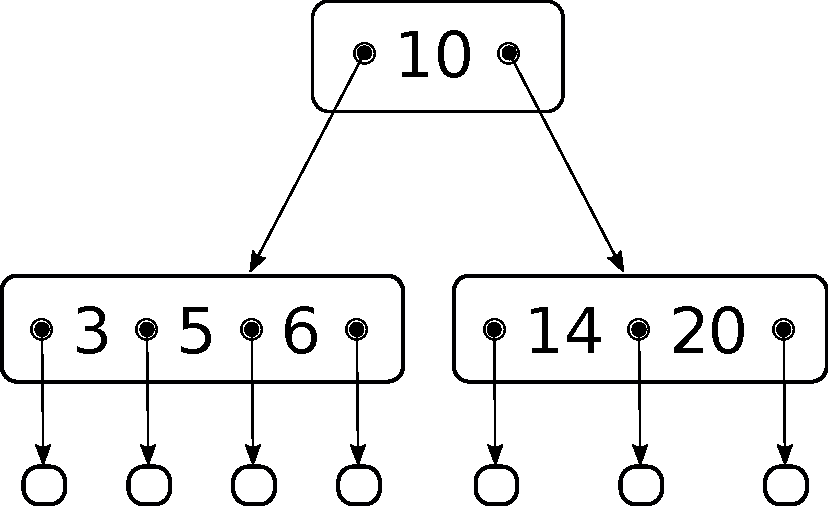
\includegraphics[width=0.5\linewidth]{btree-basic-nopair.pdf}
    \caption[Visualization of a \btree]
    {Nodes contain several elements, the internal list/array structure is not depicted.
    The dotted lines represent links to following leaf nodes that are not present in the algebraic formulation.}
    \label{fig:btree-basic}
\end{figure}


Every node \emph{Node} [($t_1$,$a_1$), …, ($t_n$,$a_n$)] $t_{n+1}$ contains an interleaved list of \textit{keys} $a_i$ and \textit{subtrees} $t_i$.
We speak of $t_i$ as the subtree to the left of $a_i$ and
the $t_{i+1}$ as the subtree to the right of $a_i$.
We refer to $t_{n+1}$ as the \textit{last} subtree.
The leafs \emph{Leaf} [$v_1$, …, $v_n$] contain a list of \textit{values} $v_i$.
Separators are only used for navigation within the tree.
The concatenation of lists of values of a tree $t$ yield
all elements contained in the tree, we refer to this list as \emph{leaves t}.
A \btree\ with above structure must fulfill the properties
\textit{balancedness}, \textit{order} and \textit{alignment}.

\textbf{Balancedness} requires
that each path from the root to a leaf has the same length.
In other words, the height of all trees in one level of the tree must be equal,
where the height is the maximum path length to a leaf.

The \textbf{order} property ensures a minimum and maximum
number of subtrees for each node.
A \btree\ is of order $k$, if each internal node has at least $k+1$
subtrees and at most $2k+1$.
The root is required to have a minimum of 2 and a maximum of $2k+1$ subtrees.
We require that $k$ be strictly positive, as for $k = 0$ the requirements on the tree
root are contradictory.

\textbf{Alignment} means that keys are sorted with respect to separators:
For a separator $k$ and all keys $l$ in the subtree to the left, $l < k$,
and all keys $r$ in the subtree to the right, $k \leq r$.
(where $\leq$ and $<$ can be exchanged).

\begin{lstlisting}[mathescape=true, language=Isabelle,label=lst:btree-alignment-def]
fun inbetween where
  inbetween f l [] t u = f l t u |
  inbetween f l ((sub,sep)#xs) t u = (f l sub sep $\wedge$ inbetween f sep xs t u)

fun aligned where
  aligned l (Leaf ks) u = (l < u $\wedge$ ($\forall$x $\in$ set ks. l < x $\wedge$ x $\le$ u)) |
  aligned l (Node ts t) u = (inbetween aligned l ts t u)
\end{lstlisting}


Note that this property cannot be reduced to the sortedness of an inorder traversal,
because whether or not an element is allowed to be equal to a separator or not
depends on the precise relative position within the tree, not only on its position in the traversal.
Moreover the separator to the right of its preceding separator must be smaller,
implying sortedness of all lists within nodes.
For the elements within the leaves, \textbf{sortedness} is required explicitely.
We show the even stronger fact that \emph{leaves t} is sorted.
This is a useful statement when arguing about the correctness of of set operations.
% is used in the abstract proofs to
% argue about the correctness of tree operations to refine set operations
% based on the list view on their elements
% as described by Nipkow \cite{DBLP:conf/itp/Nipkow16}.

The finally obtained efficient implementation of \btrees\ is defined
on the imperative level.
Each imperative node contains pointers (\emph{ref}) rather than the full subtree and
stores all values in partially filled arrays (\emph{pfarray}) rather than lists.
Other than that the data structures are refined to an imperative level,
each imperative node contains the equivalent information to an abstract node.
The only addition is that leafs now also contain a pointer to another leaf,
which will form a linked list over all leafs in the tree.

\begin{lstlisting}[mathescape=true, language=Isabelle,label=lst:btree-imp-def]
datatype 'a btnode =
  Btnode (('a btnode ref option * 'a) pfarray) ('a btnode ref) |
  Btleaf ('a pfarray) ('a btnode ref option)
\end{lstlisting}

With this setup, it is possible to modify elements on the heap and share pointers.
In order to use the algebraic data structure as a reference point,
we introduce a refinement relation.
The correctness of operations on the imperative node
can then be shown by relating imperative input and output
and to the abstract input and output of a correct abstract operation.
In particular we want to show that if we assume \emph{R t $t_i$},
where $R$ is the refinement relation and $t$ and $t_i$ are the abstract
and the imperative version of the "same" tree,
\emph{R o(t) $o_i$($t_i$)} should hold, where $o_i$ is the imperative refinement
of operation $o$.

The relation is expressed as a separation logic formula that links an abstract tree to its
imperative equivalent.
The notation for separation logic in Isabelle is quickly summarized in the list below.
\begin{itemize}
    \item \textit{emp} holds for the empty heap
    \item \textit{true} and \textit{false} hold for every and no heap respectively
    \item $\uparrow(P)$ holds if the heap is empty and predicate $P$ holds
    \item $a \mapsto_r x$ holds if the heap at position $a$ is reserved and contains
    value $x$ where $x$ is of some type $'a::heap$
    \item $\exists_A x.\ P\ x$ holds if there exists some $x$ such that predicate P
    holds on the heap for given $x$.
    \item $P_1 * P_2$ denotes the separting conjunction and holds if each assertion $P_1$ and $P_2$ hold on non-overlapping parts
    of the heap
    \item \emph{is\_pfa c xs xsi} expresses that $xsi$ is a partially filled array
    with capacity $c$ that refines the list $xs$.
    \item \emph{list\_assn P xs ys} expresses that \emph{P xs[i] ys[i]} holds for all $i \leq |xs| = |ys|$.
\end{itemize}
% TODO introduce notation of sep logic
More details can be found in the work of Lammich. \cite{DBLP:journals/afp/LammichM12}

The function relates an algebraic tree (\emph{bplustree})
and an imperative tree (\emph{btnode ref}), as well as the first and last leaf of the imperative tree.
The relation states that all parts of the abstract tree
are refined by the imperative tree.
The abstract list is itself refined by an array,
and the pointers on subtrees refine again the subtrees of the algebraic tree.

\begin{lstlisting}[mathescape=true, language=Isabelle,label=lst:btree-relation]
fun bplustree_assn :: nat $\Rightarrow$ 'a bplustree $\Rightarrow$ 'a btnode ref $\Rightarrow$ 'a btnode ref $\Rightarrow$ 'a btnode ref
    where
  bplustree_assn k (LNode xs) a r z =
  $\exists_A$ xsi fwd.
      a $\mapsto_r$ Btleaf xsi fwd
    * is_pfa (2*k) xs xsi
    * $\uparrow$(fwd = z)
    * $\uparrow$(r = Some a)
    |
  bplustree_assn k (Node ts t) a r z =
  $\exists_A$ tsi ti tsi' rs.
      a $\mapsto_r$ Btnode tsi ti
    * is_pfa (2*k) tsi' tsi
    * $\uparrow$(length tsi' = length rs)
    * list_assn (($\lambda$ t (ti,r',z'). bplustree_assn k t (the ti) r' z') $\times_a$ id_assn) ts (
        zip (zip (map fst tsi') (zip (butlast (r#rs)) rs))) (map snd tsi')))
    * bplustree_assn k t ti (last (r#rs)) z)
\end{lstlisting}

The first and last leaf are used to express the structural invariant
that the leafs are correctly linked.
This property will allow obtaining the iterator on the tree in \autoref{sec:imperative_iter}.
There is no abstract equivalent for the next pointers in the leafs,
therefore we can only introduce and reason about this invariant on the imperative layer.
Due to the constraints of separation logic, we can also not express this invariant
in a separate statement from the refinement relation.
We need to access the keys in each node to ensure the refinement relation,
and in this step we also access the memory that contains the next pointers.
Since separation logic only permits us to access the memory location
exclusively in each term separated by the separating conjunction, this access 
must both cover the keys and their refinement relationship as well as the next pointer
and the corresponding structural invariant.

The structural invariant is ensured
by passing the first leaf of the right neighbor to each subtree.
We obtain these leafs not by explicitly computing them.
Functions that follow the pointers of the tree are not guaranteed
to terminate without the context of the structural soundness of the tree,
which is only established within the relationship.
Instead, we assume that there exists a list of such leaf pointers using an existential quantifier.
We ensure that this list is the correct one, by passing the supposedly
first leafs into each subtree.
The pointer is passed recursively to the leaf node,
where it is compared to the actual pointer of the leaf.

\subsection{Node internal navigation}
\label{sec:split}

In order to define meaningful operations that navigate
the node structure of the \btree,
we need to find a method that handles search within a node.
On binary trees, this question is simple, in each node we either choose
the left or right subtree.
For general $k$-ary \btrees\ there have not been sophisticated search strategies.
Ernst \cite{DBLP:journals/sosym/ErnstSR15} and Malecha \cite{DBLP:conf/popl/MalechaMSW10}
both use a linear search through the node lists.
However, \btrees\ are supposed to have memory page sized nodes \cite{DBLP:journals/csur/Comer79}, 
which makes a linear search unfeasible in practical contexts.

We introduce a context (\emph{locale} in Isabelle) in which we assume that we
have access to a function that correctly navigates through the node internal structure.
We call this function \emph{split}, and define it only by its behavior.
Given a list of separator-subtree pairs and a search value $x$, the function should return the pair $(s,t)$ such that,
according to the structural invariant of the \btree, $t$ must contain $x$ or will hold $x$ after a correct insertion.
A corresponding function \emph{split\_list} is defined on the separator-only lists in the leaf nodes.

In the following sections, all operations are defined and verified
based on \emph{split} and \emph{split\_list}.
Finally, when approaching imperative code extraction,
we provide a binary search based function, that refines \emph{split}.
This binary search is directly implemented and verified on the imperative
level and is eventually plugged into the abstractly defined
imperative operations on the \btree.
Thus we obtain imperative code that makes use of an efficient
binary search, without adding complexity to the proofs.
The definition and implementation closely follows
the approach described in detail in the
verification of B-Trees \cite{DBLP:journals/afp/Mundler21}.
% TODO copy from BSc. Thesis?


\section{Set operations}
\label{sec:set}

\btrees\ refine abstract sets on linearly ordered elements.
For a tree $t$, the refined abstract set is computed as \emph{set (leaves t)}.
The set interface requires that there should be query, insertion and deletion
operations $o_t$ such that \emph{set (leaves ($o_t$ t)) = o (set (leaves t)}.
Moreover, the invariants described in \autoref{sec:approach}
can be assumed to hold for $t$ and are required for $o_t$.
We provide these operations and show there correctness on the functional
layer first, then refine the operations further to the imperative
layer.
For point queries and insertion, we follow the implementation
suggested by Bayer \cite{DBLP:journals/acta/BayerM72}.

\subsection{Functional Point Query}
\label{sec:functional_pq}

For an inner node $t$ and a searched value $x$, find the correct subtree $s_t$
such that if a leaf of $t$ contains $x$, a leaf of $s_t$ must contain $x$.
Then recurse on $s_t$.
Inside the leaf node, we search directly in the list of values.
Note that we assume here that a \textit{split} and \textit{isin\_list} operation exist,
as described in \autoref{sec:split}.

\begin{lstlisting}[mathescape=true, language=Isabelle,label=lst:isin-def]
fun isin:: "'a bplustree $\Rightarrow$ 'a $\Rightarrow$ bool" where
  isin (LNode ks) x = (isin_list x ks) |
  isin (Node ts t) x = (case split ts x of
     (_,(sub,sep)#rs) $\Rightarrow$ isin sub x
   | (_,[]) $\Rightarrow$ isin t x
  )
\end{lstlisting}

Since this function does not modify the tree involved at all,
we only need to show that it returns the correct value.

\begin{lstlisting}[mathescape=true, language=Isabelle,label=lst:isin-set-inorder]
theorem isin_set_inorder:
  assumes "sorted_less (leaves t)"
    and "aligned l t u"
  shows "isin t x = (x $\in$ set (leaves t))"
\end{lstlisting}

In general these proofs on the abstract level are made
based on another refinement relation suggested by Nipkow. \cite{DBLP:conf/itp/Nipkow16}
In this relation, we say that the \btree\ $t$ refines a sorted list of its leaf elements, \emph{leaves t}.
We argue that recursing into a specific subtree
is equivalent to splitting this list at the correct position
and searching in the correct sublist.
The same approach was applicable for proving the correctnes of functional
operations on B-Trees. \cite{DBLP:journals/afp/Mundler21}

The proofs on the functional level can therefore be made concise.
We go on and define an imperative version of the operation that
refines each step of the abstract operation to equivalent operations on the imperative tree.

\subsection{Imperative Point Query}
\label{sec:imperative_pq}

The imperative version of the point query is a partial function.
Termination can not be guaranteed anymore,
at least without further assumptions.
This is inevitable since the function would not terminate
given cyclic trees.
However, we will show that if the input refines an abstract tree,
the function terminates and is correct.

\begin{lstlisting}[mathescape=true, language=Isabelle,label=lst:isin-imp-def]
partial_function (heap) isin :: "'a btnode ref $\Rightarrow$ 'a $\Rightarrow$  bool Heap" where
  isin p x = do {
  node $\leftarrow$ !p;
  (case node of
     Btleaf xs _ $\Rightarrow$ imp_isin_list x xs |
     Btnode ts t $\Rightarrow$ do {
       i $\leftarrow$ imp_split ts x;
       tsl $\leftarrow$ length ts;
       if i < tsl then do {
         s $\leftarrow$ get ts i;
         let (sub,sep) = s in
           isin (the sub) x
       } else
           isin t x
    }
)}
\end{lstlisting}

Again, we assume that \emph{imp\_split} does the correct node internal search operations
and refines an abstract \emph{split}.
Note how \emph{imp\_split} does not actually split
the internal array, but rather returns the index of the pair
that would have been returned by the abstract split function.
The pattern matching against a an empty list
is replaced by comparing the index to the length of the list $l$,
where the last subtree is signalled by returning $l$.

In order to show that the function returns the correct result,
we show that it does the same operation on the imperative tree
as on the algebraic tree.
This is expressed in Hoare Triple notation and Separation Logic.

\begin{lstlisting}[mathescape=true, language=Isabelle,label=lst:isin-refines]
lemma  
   assumes "k > 0" and "root_order k t"
    and "sorted_less (inorder t)" and "sorted_less (leaves t)"
   shows
   "<bplustree_assn k t ti r z>
     isin ti x
   <$\lambda$y. bplustree_assn k t ti r z * $\uparrow$(isin t x = y)>$_t$"
\end{lstlisting}

The proof follows inductively on the structure of the abstract tree.
Assuming structural soundness of the abstract tree refined by the pointer passed in ,
the returned value is equivalent to the return value of the abstract function.
We must explicitely show that the tree on the heap
still refines the same abstract tree after the operation,
which was implicit on the abstract layer.
It follows directly, since no operation in the imperative
function modifies part of the tree.

\subsection{Insertion and Deletion}
\label{sec:insert_delete}

The insertion operation and its proof largely line up with the approach to point queries.
But since insertion modifies the tree,
we need to additionally show on the abstract level that the modified tree
maintains the invariants of \btrees.

On the imperative layer, we show that the heap state
after the operation refines the tree
after the abstract insertion operation.
It follows that the imperative operation
also maintains the abstract invariants.
Moreover, we need to show that the leaf pointers
maintain correct linking after the operation.
This can only be shown on the imperative level as there is no abstract equivalent
to the shared pointers.

\begin{lstlisting}[mathescape=true, language=Isabelle,label=lst:insert-refines]
lemma insert_rule:
    assumes "k > 0" "sorted_less (inorder t)" "sorted_less (leaves t)" "root_order k t"
    shows
    "<bplustree_assn k t ti r z>
    imp_insert k x ti
    <\<lambda>u. bplustree_assn k (insert k x t) u r z>\<^sub>t"
\end{lstlisting}
  

Deletion is less commonly implemented and even less verified,
however we provide a verified functional definition of deletion and a definition of an imperative refinement.
Showing the correctness of the imperative version would largely follow
the same pattern as the proof of the correctness of insertion.
The focus of this work is not on basic tree operations
however, but on obtaining an iterator view on the tree.


\section{Range operations}
\label{sec:range}

On the functional level, the forwarding leaf pointers in each leaf
are not present, as this would require aliasing.
Therefore, the abstract equivalent of an iterator
is simply a concatenation of all leaf contents by
trivially copying them together recursively.
%Range iterators then concatenate the correct parts of the abstract tree.
When refining the operations, we will make use of the leaf pointers
to obtain an efficient implementation.

\subsection{Iterators}
\label{sec:imperative_iter}

Implementing an iterator over the leafs of a \btree\ is simple.
We recurse down the tree to obtain the first leaf.
From there we follow leaf
pointers along the skirt of the tree until we reach the final leaf marked by a null next pointer.
However, from an assertion perspective the situation is more intricate.
It is important to find an explicit formulation of the linked list view on the leaf pointers.
Meanwhile, we want to maintain enough information about the remainder of the tree
to be able to reconstruct the assertion about the whole tree.
We cannot simply express the linked list view and the view on the
whole tree at the same time,
as separation logic forces us to not make statements about the contents of
any memory location twice.
This is an important feature of separation logic,
in order to keep the parts of the heap disjunct and
thus be able to locally reason about the heap state.

We therefore follow the approach of \cite{DBLP:conf/popl/MalechaMSW10} and
try to find an equivalent formulation that separates the whole tree in a
view on its inner nodes and the linked leaf node list.
The central idea to separate the tree is to
express that the linked leaf nodes refine \emph{leaf\_nodes t}
and that the inner nodes refine \emph{trunk t}, as depicted in \autoref{fig:btree-view-split}.
These are two independent parts of the heap and therefore
the statements can be separated using the separating conjunction.

However, a first attempt to use the below relationship fails.
The reason is that we cannot express that the linked leaf nodes
are precisely the leaf nodes that the lowest level of inner nodes point to.
We can show that the whole tree can be separated into a linked list in the leafs
and some remainder of the heap, but we cannot show that we can necessarily transform
these two statements back together and obtain a structurally consistent \btree.

\begin{lstlisting}[mathescape=true, language=Isabelle,label=lst:btree-view-split-oneway]
lemma bplustree_leaf_nodes:
  "bplustree_assn k t ti r z $\Longrightarrow_A$ leaf_nodes_assn k (leaf_nodes t) r z * true"
\end{lstlisting}

% TODO graphic explaining the issue
\begin{figure}
    \centering
    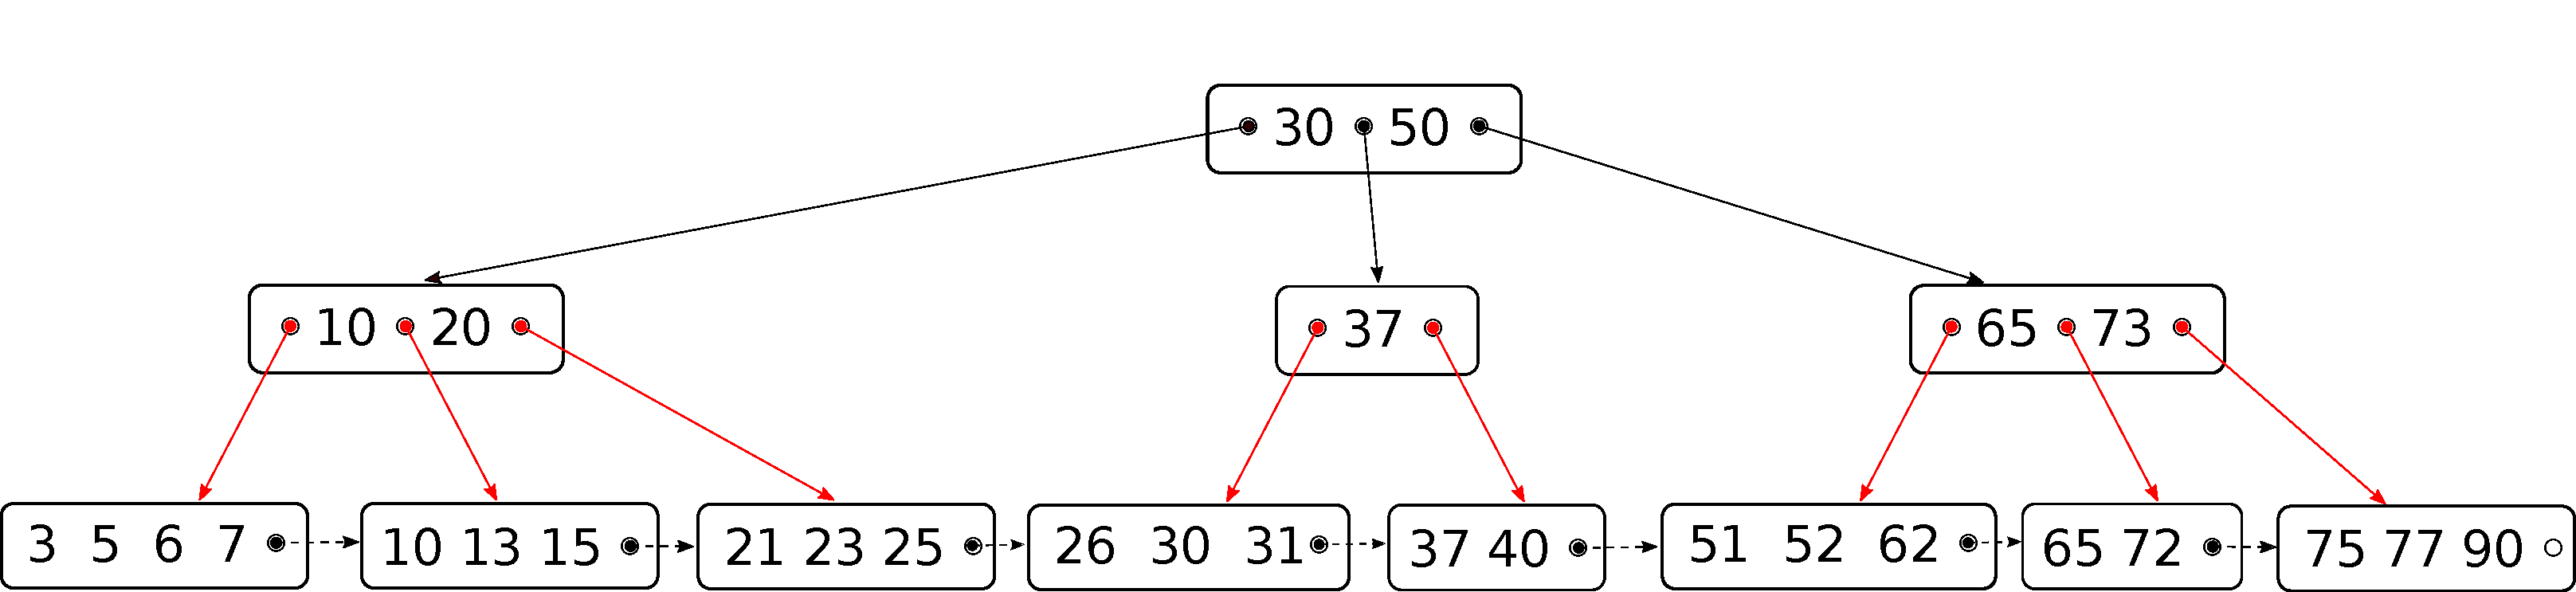
\includegraphics[width=1\linewidth]{btree-view-split.pdf}
    \caption[Split view of the \btree]
    {In order to obtain separate assertions about the concatenated leaf list (\emph{leaf\_nodes})
    and the internal nodes (\emph{trunk}) of the tree, the structure is abstractly split along the
    pointers marked in red, the \emph{fringe}. In order to be able to combine the \emph{leaf\_nodes} and the \emph{trunk} together,
    the \emph{fringe} has to be extracted and shared explicitely.}
    \label{fig:btree-view-split}
\end{figure}

The root of this problem is actually a feature of the refinement approach.
When stating that a part of the heap
refines some abstract data structure,
we make no or little statements about concrete memory locations or pointers.
This is useful, as it reduces the size of the specification
and the proof obligations.
In this case it gets in our way.

% vis?

We cannot express that the lowest pointers
in the internal node hierachy refine the leafs
that we refine in the leaf list,
as this would violate the disjunctness of heaps.
Even if we did, this statement would not be strong enough
to guarantee that the actual memory locations
are the same.
We need to specifically denote that these pointers,
and not the structure they refine,
are shared between the two statements.

In a second attempt we succeed by making the sharing explicit.
We extract from the whole tree the precise list of pointers to leaf nodes, the \emph{fringe}
in the correct order as visualized in \autoref{fig:btree-view-split}.
We express this new view by extending the existential quantifier in \autoref{lst:btree-relation}
to assume that there is a partition of the \emph{fringe},
distributing the pointers correctly on each subtree.
The resulting assertion can be seen in \autoref{fig:btree-assn-leafs}.
A convenient fact is that the view on the tree that makes \emph{fringe} explict
is equivalent to the view where we do not the pointers precisely.
The statement from \autoref{lst:btree-relation} is strong enough to guarantee that such a list exists.
Using the \emph{fringe}, we can precisely state an equivalent separated assertion.

\begin{lstlisting}[mathescape=true, language=Isabelle,label=lst:btree-extract-leafs]
lemma bplustree_extract_leafs:
    "bplustree_assn k t ti r z = ($\exists_A$fringe. bplustree_assn_leafs k t ti r z fringe)"
\end{lstlisting}


\begin{figure}
    \centering
\begin{lstlisting}[mathescape=true, language=Isabelle,label=lst:btree-assn-leafs]
fun bplustree_assn_leafs where
    bplustree_assn_leafs k (LNode xs) a r z fringe =
   ($\exists_A$ xsi fwd.
        a $\mapsto_r$ Btleaf xsi fwd
      * is_pfa (2*k) xs xsi
      * $\uparrow$(fwd = z)
      * $\uparrow$(r = Some a)
      * $\uparrow$(fringe = [a])
    ) |
    bplustree_assn_leafs k (Node ts t) a r z fringe =
   ($\exists_A$ tsi ti tsi' tsi'' rs split.
        a $\mapsto_r$ Btnode tsi ti
      * bplustree_assn_leafs k t ti (last (r#rs)) (last (rs@[z])) (last split)
      * is_pfa (2*k) tsi' tsi
      * $\uparrow$(concat split = fringe)
      * $\uparrow$(length tsi' = length rs)
      * $\uparrow$(length split = length rs + 1)
      * $\uparrow$(
          tsi'' = zip (zip (map fst tsi') (zip (butlast (r#rs))
          (zip rs (butlast split)))) (map snd tsi')
        )
      * list_assn (
          ($\lambda$ t (ti,r',z',fring). bplustree_assn_leafs k t (the ti) r' z' fring)
           $\times_a$ id_assn
        ) ts tsi''
      )
\end{lstlisting}
    \caption[Definition of extracted leafs assertion]{
        In order to be able to correctly relate leaf view and internal nodes,
        the shared pointers have to be made explicit without accessing them.
        For this reason, a refined version of the tree assertion is derived
        that guarantees to include the pointers passed as $leafptrs$.
    }
    \label{fig:btree-assn-leafs}
\end{figure}


In the separated view, we now require that the \emph{fringe} is
precisely the list of pointers in the linked list \emph{leaf\_nodes}.

\begin{lstlisting}[mathescape=true, language=Isabelle,label=lst:btree-view-split]
lemma bplustree_leaf_nodes_sep:
  "bplustree_assn_leafs k t ti r z fringe =
   leaf_nodes_assn k (leaf_nodes t) r z fringe * inner_nodes_assn k t ti r z fringe"
\end{lstlisting}


In the work of Malecha \cite{DBLP:conf/popl/MalechaMSW10}, 
this list of precise leaf pointers is exactly the list of abstract leafs,
as the abstract leafs each contain the precise heap pointer they are refining.
Keeping the two layers separate leads to the need of specifying
exactly where the actual pointers are relevant
and where it is enough to know that the allocated memory refines
an abstract tree.

Now to obtain an iterator on the leaf nodes of the tree,
we simply obtain the first leaf by a recursive function, leaving
us with a tree refining an abstract tree and the pointer to its first leaf.

\begin{lstlisting}[mathescape=true, language=Isabelle,label=lst:btree-first-leaf]
lemma first_leaf_rule:
  assumes "k > 0" and "root_order k t"
  shows "<bplustree_assn k t ti r z>
  first_leaf ti
  <$\lambda$u. bplustree_assn k t ti r z * $\uparrow$(u = r)>$_t$"
\end{lstlisting}


On the result, we can apply the view split from \autoref{lst:btree-view-split}
to realize that we now have a pointer that provides a list-recursive
view on the leaf elements and the inner nodes on the remaining heap.
In a next step, we show that such a list view can be used
to define an imperative iterator fulfilling the list iterator interface from Lammich. \cite{DBLP:conf/itp/Lammich19}
Starting from the root of the tree and an assertion on the integrity
of the whole tree,
we have now obtained an iterator on the leaf nodes.
This iterator assertion must already contain
the remaining assertion on the internal nodes of the tree.
The reason is that this way, the iterator
can be used to obtain knowledge about the whole
original tree again at the end of the iteration.
Also, this conveniently hides the complexity
of more assertions away from the client.

To really obtain an iterator that returns every single element of the
leaf nodes, rather than the leaf nodes or the contained arrays themselves,
we introduce a flattening iterator.
It takes an outer iterator over a data structure \textit{a} that returns elements of type \textit{b},
and inner iterator over the data structure \textit{b}.
The result is instantiated code that refines an iterator
over the concatenated list of elements refined by the outer iterator.

Using this structure, we obtain a function that creates an iterator
over the leaf elements of the original tree.
Note how all notion of the explicitely shared leaf pointers
has disappeared on this level, as their existence was hidden within the definition
of the leaf elements iterator.

\begin{lstlisting}[mathescape=true, language=Isabelle,label=lst:btree-view-split]
lemma leaf_elements_iter_init_rule:
  assumes "k > 0" and "root_order k t"
  shows "<bplustree_assn k t ti r None>
    leaf_elements_iter_init ti
    <$\lambda$it. leaf_elements_iter k t ti r (leaves t) it>$_t$"
\end{lstlisting}

\subsection{Range queries}
\label{sec:imperative_range}

A common use case of \btrees\ 
is the obtaining of a lower bound on some key
or to obtain  all elements within a certain range. \cite{DBLP:journals/ftdb/Graefe11}
A lower bound and the beginning of such a range iterator
can be both obtained in logarithmic time, making use of the tree structure.
The operation is similar to the point query operation,
only that it does not return the
found element but an iterator pointing to this element.
The range bounded from below is all elements returned by the iterator,
the first element being the lower bound.

\begin{lstlisting}[mathescape=true, language=Isabelle,label=lst:btree-lrange]
fun lrange:: "'a bplustree $\Rightarrow$ 'a $\Rightarrow$ 'a list" where
    lrange (LNode ks) x = (lrange_list x ks) |
    lrange (Node ts t) x = (
        case split ts x of (_,(sub,sep)#rs) $\Rightarrow$ (
               lrange sub x @ leaves_list rs @ leaves t
        )
     | (_,[]) $\Rightarrow$ lrange t x
    )
\end{lstlisting}
  
Again, we assume that there exists a function \textit{lrange\_list} that
obtains the lower bounded range from a list of sorted elements.
Note how the abstract function explicitely recurses into
remaining parts of the tree and constructs lists on the leaves by concatenating them.
This will not be the case in the refined version anymore
as we know that the iterator comprises all elements in the remainder of the tree.

However showing this turns out to be not as straightforward
as expected, exactly due to this recursive step.
The reason is that iterators can only be expressed on a complete tree,
where the last leaf is explicitely a null pointer.\footnote{
    The issue is a technicality. Iterators have a \textit{has\_next} function
    that returns whether there are any remaining elements.
    In order to tell, we compare the leaf with the last leaf of the tree.
    If this is a valid leaf node (not a null pointer) we need to show
    that the linked leaf list is not cyclic - a proof obligation
    that can be omitted in the linked list view.
    % TODO more precise?
}
This contrasts the linked list view on the leafs that can be expressed
recursively on subtrees.

Therefore we introduce an alternative formulation of the
abstract function, similar in thought to how we obtained the iterator
on the list from the first leaf of the tree.
In a first step, we obtain the correct list of leaf nodes
based on the recursive search through the tree.
In a second step, we obtain the head of the list and apply
the function that returns the lower bounded range of elements within,
and concatenate it with the tail of the returned list of leaf nodes.
This way, during refinement of the tree internal search
we only use the linked list view and the internal node view.
Only when we have obtained the correct list for the whole tree,
where the last element is a null pointer,
we transform the result into the leaf element iterator.

\begin{lstlisting}[mathescape=true, language=Isabelle,label=lst:btree-leafs-range]
lemma concat_leafs_range_rule:
    assumes "k > 0" and "root_order k t" 
    and "sorted_less (leaves t)" and "Laligned t u"
    shows 
 "<bplustree_assn k t ti r None>
  concat_leafs_range ti x
  <leaf_elements_iter k t ti r (lrange t x)>$_t$"
\end{lstlisting}

% TODO vis


\section{Conclusion}
\label{sec:conclusion}

During writing, this project mainly comprised two parts.
The first part was rather theoretical,
trying to figure out the best, if any, appraoch
to express statements about the abstract tree and operation,
their imperative equivalent and
the refinement relationship between them.
The second part was their verification,
which went rather smooth on the abstract level but induced much headache
on the imperative reasoning level.
Since all functional correctness concerns are covered by
the refinement relation, all that remains
to show is that the refinement relation holds,
and this process is very technical
and mainly requires justification of thousands of small
implementation details.
However, we can imagine that this is no comparison
to the headache induced by having to show
functional correctness on the imperative level as well.

\subsection{Lessons learnt}

Handling assertions has always been
a bit tedious throughout the project.
A major alleviation was the introduction of a specialized tool
that would substitute multiplicative terms in the formular
regardless of the disctribution in the original term.
This way, we could substitute equivalent assertions comprising
multiple terms, like the combination of leaf view and trunk view,
with ease.

What is currently missing in the implementation of the entailment
solving tool, is that terms that could already be derived
would be removed in an intermediate proof state.
This could be much like the simplifier in Isabelle removes terms in equation that could
already be shown to be equivalent and leaves only the remaining subterms.
This way, if the tool could verify an entailment relation holds,
all subterms remained and it was up to the proof reader
to find non-matching terms in the (potentially huge)
assertions that should match up.

On a side note, it was interesting to notice that it is rather complicated
to even express, not to speak of attempting to prove acyclicity
 along the leaf nodes of the tree, as soon as the linked list was converted into an iterator.
Fortunately, we found a way around this issue, by only considering
the complete list of nodes whenever we turned them into
iterators. In that case, they were terminated by \textit{None}
which we could guarantee not to occur earlier in the list.

\subsection{Evaluation}


The \btree\ implemented by Ernst \cite{DBLP:journals/sosym/ErnstSR15} features point queries and insertion,
however explicitely leaves out pointers within the leaves,
which forbids the implementation of iterators.
This work is closer in nature to the \btree\ implementation by Malecha \cite{DBLP:conf/popl/MalechaMSW10}.
In addition to the functionality provided in their work, we extend
the implementation with the missing Range iterator
and supply a binary search within nodes, as well as a modular approach
to further substitutionss.

With respect to the effort in lines of code and proof
as depicted in \autoref{fig:proof-comparison}, we see
that our approach is similar in effort to the approach by Malecha.
The numbers do not include introduced pure ML proof tactics.
It should be also noted that this includes the statistics
for the additional binary search and range iterator,
that make up around 1000 lines of proof each.
The comparison with Ernst is difficult, as it completely
avoids the usage of leaf pointers and the iterator
that makes up a signifant amount of the proof
with at least 1000 lines of proof on its own, and also
strongly affecting the verification of point and insertion queries
due to the additional invariant on the imperative level.
We conclude that the Isabelle/HOL framework
provides a feature set
such that verification of \btrees\ is both feasible
and comparable in effort to using Ynot or KIV/TVLA.
The strict separation of a functional and imperative
implementation yields the challenge
of potentially having to make sharing explicit.
On the other hand, it permits great freedom
regarding the actual refinement on the imperative level,
that eventually enabled
implementing functionality that is closer
to real world implementations in this work

\begin{figure}
    \centering
    \begin{tabular}{l|c|c|c}
        \                & \cite{DBLP:conf/popl/MalechaMSW10}$^{+}$ & \cite{DBLP:journals/sosym/ErnstSR15}$^{d}$ & Our approach$^{+}$ \\
        \hline
        Functional code &   360      & -                    & 413  \\ %TODO update
        Imperative code &   510      & 1862                  & 1093  \\
        Proofs          &  5190      & 350 + 510 + 2940\footnotemark[3] & 8663 \\
        Timeframe (months) &  -     & 6+                      & 6\footnotemark[4] + 6   \\
    \end{tabular}
    \caption[Comparison of (unoptimized) Lines of Code and Proof and time investment in related mechanized \btree\ verifications.]
    {Comparison of (unoptimized) Lines of Code and Proof and time investment in related mechanized \btree\ verifications.
    All approaches are comparable in effort, taking into account implementation specifics.
    The marker $^d$ denotes that the implementation verifies deletion operations, whereas $^+$ denotes the implementation of iterators.
    }
    \label{fig:proof-comparison}
\end{figure}
\footnotetext[3]{
    The proof integrates TVLA and KIV, and hence comprises
    explicitely added rules for TVLA (the first number),
    user-invented theorems in KIV (the second number)
    and "interactions" with KIV (the second number).
    Interactions are i.e. choices of an induction variable, quantifier instantiation
    or application of correct lemmas.
    We hence interpret them as each one apply-Style command and hence
    one line of proof.
}
\footnotetext[4]{
    6 months include the preceding work on the verification
    of simple B-Trees.
    As they share much of the functionality with \btrees\ 
    but required their own specifics,
    the time spent on them cannot be accounted for 1:1.
}

\subsection{Future Work}

This work extends the canon on verified \btree
implementations.
Some additional features will be necessary for
usage in real-life scenarios.

A small addition to provide a true
range query can be provided by wrapping the lower-bounded
range iterator with an iterator
that stops iteration when the next element
would exceed the upper bound.

Further, this work is still lacking a verified imperative version
of the deletion function.
We already provided an abstract specification
and an imperative refinement and have seen
that all araising issues are along the lines
of the proof obligations in the refinement
proofs of point queries and insertion.

One important step towards efficient
\btree\ implementations that can be deployed
in realistic scenarios, is the migration of this code
to Isabelle-LLVM. \cite{DBLP:conf/itp/Lammich19}
At the beginning of this work, the code generator did
not yet support recursive data structures, but since
this functionality was added recently \btrees\ would be an interesting application.
Expectedly, the main difference will be the usage of Bitwords
instead of unbound natural numbers.

Finally, \btrees\ are supposed to write the contained
memory out to disk in order to maintain the durability constraint
usually required for databases.
This implementation lacks any interaction with IO systems.
We expect the formalization of correct interaction 
to be a particulary tricky task.

% TODO some analysis of the code generated? even necessary?

\bibliography{lipics-v2021-bplustrees}

\end{document}
